\documentclass[10pt,conference]{IEEEtran}

\usepackage{cite}
\usepackage{amsmath}
\usepackage{amssymb}
\usepackage{amsfonts}
\usepackage{algorithmic}
\usepackage{graphicx}
\usepackage{textcomp}
\usepackage{xcolor}
\usepackage{booktabs}
\usepackage{array}
\usepackage{url}
\usepackage{hyperref}
\usepackage{tikz}
\usetikzlibrary{arrows.meta,positioning,shapes.geometric,fit,backgrounds}

\hypersetup{
  colorlinks=true,
  linkcolor=blue,
  urlcolor=blue,
  citecolor=blue
}

\def\BibTeX{{\rm B\kern-.05em{\sc i\kern-.025em b}\kern-.08em
    T\kern-.1667em\lower.7ex\hbox{E}\kern-.125emX}}

\begin{document}

\title{Intersection of Quantum Computing and Cybersecurity: Open-Source
Reference Implementations of the NIST Post-Quantum Cryptography Standards}

\author{
\IEEEauthorblockN{Christian Kane, Venky Kottapalli, Philip Marshall}
\IEEEauthorblockA{Department of Computer Science and Engineering \\
Texas A\&M University \\
College Station, TX, USA}
}

\maketitle

\begin{abstract}
Large-scale quantum computers threaten the public-key cryptography that
secures nearly all modern digital infrastructure: Shor's algorithm reduces
the integer-factorization and discrete-logarithm problems underlying RSA
and elliptic-curve cryptography (ECC) from intractable to efficiently
solvable. Because adversaries can harvest encrypted traffic today and
decrypt it once sufficiently capable quantum hardware exists --- the
``harvest now, decrypt later'' threat --- the transition to
quantum-resistant algorithms is urgent even though large-scale quantum
computers do not yet exist. In 2024, the National Institute of Standards
and Technology (NIST) finalized the first three Post-Quantum Cryptography
(PQC) standards: FIPS 203 (ML-KEM), FIPS 204 (ML-DSA), and FIPS 205
(SLH-DSA). Public, spec-faithful, independently auditable implementations
of these standards remain scarce. This paper presents the design,
implementation, and verification of a from-scratch, spec-faithful Python
reference implementation of all three standards, sharing a minimal common
primitives package, together with an early-stage SystemVerilog hardware
accelerator for the shared Keccak/SHA-3/SHAKE primitive and a suite of
interactive browser-based visualizations. We describe the lattice- and
hash-based mathematics underlying each scheme, the software and hardware
system architecture, two notable correctness bugs discovered and fixed
during development, and our two-tier verification methodology built on
NIST's Automated Cryptographic Validation Protocol (ACVP) Known-Answer
Tests (KATs) and property-based testing. Our implementation passes all
568 tests across the three schemes, of which 271 are byte-for-byte NIST
ACVP vectors. We further present a cross-scheme comparison of public-key,
secret-key, and signature/ciphertext sizes across every NIST-defined
parameter set, quantifying the substantial size trade-off between
lattice-based and hash-based post-quantum signatures.
\end{abstract}

\begin{IEEEkeywords}
post-quantum cryptography, lattice-based cryptography, hash-based
signatures, Module-LWE, Module-SIS, ML-KEM, ML-DSA, SLH-DSA, FIPS 203,
FIPS 204, FIPS 205, NIST ACVP, hardware acceleration, Keccak, SHA-3
\end{IEEEkeywords}

\section{Introduction}

Modern digital infrastructure --- banking, communication, identity, and
data integrity --- rests on public-key cryptography whose security
depends on specific mathematical problems being computationally
intractable for classical computers: factoring large integers (RSA) and
computing discrete logarithms, including over elliptic curves (ECC/ECDSA,
Diffie--Hellman). These problems are not intractable in principle; they
are intractable \emph{for classical computers}. Shor's algorithm
\cite{shor1997} shows that a sufficiently large, fault-tolerant quantum
computer solves both problems in polynomial time, which would render
essentially all currently deployed public-key cryptography insecure.

Large-scale, fault-tolerant quantum computers do not yet exist, but the
threat is not merely theoretical or future-dated. Under the ``harvest
now, decrypt later'' model, an adversary can record encrypted traffic
today and simply retain it until quantum hardware capable of breaking it
becomes available. Data with long confidentiality requirements ---
medical records, government communications, long-lived credentials,
intellectual property --- is vulnerable \emph{today} to this attack, even
though no quantum computer capable of exploiting it currently exists.
This asymmetry is what makes migrating to quantum-resistant cryptography
urgent well ahead of the arrival of cryptographically relevant quantum
hardware.

Recognizing this, NIST ran a multi-year, public competition
\cite{nist-pqc} to select and standardize Post-Quantum Cryptography (PQC)
algorithms believed to resist both classical and quantum attack. In
August 2024, NIST finalized the first three PQC standards
\cite{nist-announce}:

\begin{itemize}
\item \textbf{FIPS 203 --- ML-KEM} \cite{fips203}: a Module-Lattice-Based
  Key-Encapsulation Mechanism, intended to replace Diffie--Hellman/RSA
  key exchange.
\item \textbf{FIPS 204 --- ML-DSA} \cite{fips204}: a Module-Lattice-Based
  Digital Signature Algorithm, intended to replace RSA/ECDSA signatures
  for general-purpose identity and data-authenticity use.
\item \textbf{FIPS 205 --- SLH-DSA} \cite{fips205}: a Stateless
  Hash-Based Digital Signature Algorithm, offering an entirely different
  (hash-based, rather than lattice-based) hardness assumption as a
  conservative fallback or long-term-security alternative.
\end{itemize}

Despite their significance, publicly available, pedagogically legible,
independently auditable implementations of all three standards together
remain scarce. Reference implementations that do exist are frequently
optimized C or assembly, which is appropriate for production deployment
but difficult to audit against the FIPS pseudocode line-by-line, and are
rarely accompanied by hardware exploration or interactive teaching
material.

\subsection{Project Objective}

The goal of this project is to produce an open-source, spec-faithful,
independently verifiable Python reference implementation of ML-KEM,
ML-DSA, and SLH-DSA, explicitly prioritizing \emph{auditability over
performance}, together with:

\begin{itemize}
\item validation against NIST's official ACVP Known-Answer Test vectors,
  the authoritative functional-correctness bar for FIPS-compliant PQC
  implementations;
\item an in-house property-based test suite exercising invariants the
  fixed KAT vectors do not directly target;
\item a from-scratch SystemVerilog hardware accelerator for the Keccak
  permutation shared by all three schemes' hash and extendable-output
  functions (XOFs);
\item interactive, browser-based visualizations of each scheme's
  internal structure, intended as teaching artifacts; and
\item a cross-scheme analysis of the resulting key, ciphertext, and
  signature sizes.
\end{itemize}

\subsection{Contributions}

This paper makes the following contributions:

\begin{enumerate}
\item A complete, from-scratch Python implementation of ML-KEM-768,
  ML-DSA-65, and SLH-DSA-SHAKE-128s, each mapping every module to a
  specific FIPS section and algorithm number, sharing only genuinely
  duplicated logic.
\item Verification against 271 official NIST ACVP KAT vectors plus 297
  in-house unit and property-based tests, for 568/568 passing tests
  total.
\item A documented account of two non-trivial correctness bugs
  discovered during development --- a centered-norm sign error in ML-DSA
  and a wrong XOF variant in SLH-DSA --- and the testing methodology that
  surfaced each.
\item An early-stage, cycle-accurate SystemVerilog Keccak-f[1600]/SHA-3/SHAKE
  accelerator, verified in simulation against the Python reference
  implementation's own hash wrappers.
\item Four self-contained, dependency-free interactive web visualizations
  covering all three schemes plus a cross-scheme size-comparison hub.
\item A quantitative comparison of public-key, secret-key, and
  signature/ciphertext sizes across all NIST-defined parameter sets of
  all three standards.
\end{enumerate}

The remainder of this paper is organized as follows. Section II reviews
the mathematical background --- lattice cryptography, Module-LWE/SIS, and
hash-based one-way functions --- and related work. Section III describes
our methodology, including language choice, repository conventions, and
verification strategy. Section IV presents the system architecture of
the software and hardware components. Section V details the technical
design of each algorithm and documents the bugs found during
development. Section VI presents and discusses our results. Section VII
concludes, and Section VIII outlines future work.

\section{Background and Related Work}

\subsection{The Quantum Threat to Classical Public-Key Cryptography}

RSA's security rests on the difficulty of factoring the product of two
large primes; ECC/ECDSA and Diffie--Hellman rest on the difficulty of the
discrete logarithm problem, either over $\mathbb{Z}_p^*$ or an elliptic
curve group. Both problems belong to a class Shor's algorithm solves
efficiently on a quantum computer by exploiting quantum Fourier
transforms to find the period of a modular exponentiation function
\cite{shor1997}. Grover's algorithm additionally provides a quadratic
speedup against generic search problems, weakening (but not breaking)
symmetric primitives like AES and SHA-2/SHA-3 --- which is why PQC
standardization focuses almost entirely on replacing asymmetric
primitives, while symmetric primitives are addressed simply by using
longer keys/outputs.

\subsection{Lattice Cryptography}

A lattice is an infinite, regularly repeating grid of points in
$n$-dimensional space formed by all integer combinations of a set of
basis vectors $B = \{b_1, \dots, b_n\}$:
\[
\mathcal{L}(B) = \left\{ \sum_{i=1}^{n} x_i b_i \;\middle|\; x_i \in
\mathbb{Z} \right\}.
\]
The same lattice admits many different bases. A ``good'' basis (short,
nearly orthogonal vectors) makes geometric questions about the lattice
easy to answer; a ``bad'' basis (long, skewed vectors) makes the same
questions extraordinarily hard. This basis-dependent asymmetry is the
foundation of lattice cryptography: the holder of a secret good basis (or
an equivalent trapdoor) can solve problems efficiently, while an attacker
who sees only a public bad basis cannot. As the dimension $n$ grows into
the hundreds, these problems become computationally intractable for both
classical and (so far as is known) quantum algorithms.

The two canonical hard lattice problems are the \emph{Shortest Vector
Problem} (SVP) --- find the shortest nonzero vector in the lattice --- and
the \emph{Closest Vector Problem} (CVP) --- given an arbitrary point in
space, find the lattice point nearest to it. Cryptography needs problems
that are hard \emph{on average} over randomly chosen keys, not merely in
the worst case, and that are efficient to evaluate. This motivates two
structured average-case problems, each provably as hard as worst-case
SVP/CVP under standard reductions:

\begin{itemize}
\item \textbf{Module-LWE} (Learning With Errors): hides a secret vector
  $s$ inside noisy linear equations
  \[
  b = A \cdot s + e \pmod q,
  \]
  where $A$ is a public matrix and $e$ is small structured noise. Module-LWE
  corresponds to an average-case CVP instance and underlies ML-KEM.
\item \textbf{Module-SIS} (Short Integer Solution): asks for a short
  nonzero vector $z$ satisfying
  \[
  A \cdot z \equiv 0 \pmod q
  \]
  for a public matrix $A$. Module-SIS corresponds to an average-case SVP
  instance and underlies ML-DSA.
\end{itemize}

The ``Module'' prefix indicates that $A$, $s$, $e$, and $z$ are composed
of elements of a polynomial ring $R_q = \mathbb{Z}_q[X]/(X^n+1)$ rather
than plain integers, which shrinks key sizes and accelerates arithmetic
(via the Number-Theoretic Transform, an FFT-analogue over $\mathbb{Z}_q$)
while preserving the underlying worst-case hardness guarantees
\cite{peikert}.

\subsection{Hash-Based Cryptography}

SLH-DSA takes an entirely different approach, relying only on the
security of an underlying cryptographic hash function (in our
implementation, SHAKE256) as a one-way function --- easy to compute in
one direction, infeasible to invert. Hash-based signatures compose four
primitives:

\begin{itemize}
\item \textbf{WOTS+} (Winternitz One-Time Signature+): a one-time
  signature scheme built from hash chains, secure for exactly one
  signature per key pair.
\item \textbf{XMSS}: a Merkle tree whose leaves are WOTS+ public keys,
  allowing many one-time key pairs to be authenticated under a single
  short Merkle root.
\item \textbf{A hypertree (HT)}: a multi-layer stack of XMSS trees, where
  each higher-layer tree signs the root of a tree below it, extending the
  number of one-time signatures that can be authenticated far beyond a
  single XMSS tree's leaf count.
\item \textbf{FORS} (Forest of Random Subsets): a few-time signature
  scheme used specifically to sign the (large) message digest, since
  signing an arbitrary-length hash directly with WOTS+ would be
  insecure.
\end{itemize}

Because the security of every layer reduces to hash-function properties
rather than any number-theoretic or lattice assumption, hash-based
signatures are considered a conservative fallback, resistant even to
advances in cryptanalysis that might unexpectedly weaken lattice
assumptions. SLH-DSA is \emph{stateless}: unlike earlier hash-based
schemes (e.g., XMSS or LMS used directly), the signer never has to
remember or atomically update any per-signature state, eliminating an
entire class of catastrophic key-reuse failures that arise if a stateful
scheme's counter is ever duplicated (e.g., across a virtual-machine
snapshot restore).

\subsection{Related Work}

NIST's own reference and optimized implementations, and the
pq-crystals/PQClean C reference implementations that informed the
standards, prioritize performance and constant-time execution, which
necessarily obscures the line-by-line correspondence to the FIPS
pseudocode behind manual loop unrolling, precomputed tables, and
platform-specific optimization. Several Python ports exist for individual
schemes, but a single, actively maintained repository implementing
\emph{all three} finalized standards side-by-side, with a shared minimal
primitives package, full NIST ACVP KAT coverage, and an accompanying
hardware exploration, is comparatively rare. This project is positioned
to fill that gap for auditability and pedagogy rather than deployment.

More concretely, the PQClean project \cite{pqclean} collects
cross-vetted, portable C reference implementations of many PQC schemes,
including ML-KEM, ML-DSA, and SLH-DSA, and is itself the ancestor of
several bindings into higher-level languages; the Open Quantum Safe
project's \texttt{liboqs} \cite{liboqs} wraps these (and other candidate)
implementations behind a single C API and integrates them into forks of
OpenSSL and other TLS libraries for experimentation. Both projects are
outstanding engineering references, but neither one targets our specific
goal: a reference whose \emph{primary} audience is a human reader
checking correctness against the FIPS pseudocode section by section,
rather than a downstream consumer linking against a stable ABI. Our
choice of Python over C, our insistence that every module cite its FIPS
algorithm number in its docstring, and our explicit non-goal of
constant-time or performance hardening are all direct consequences of
optimizing for that different audience. Where PQClean and liboqs answer
``how do I use this in a real system,'' our repository is built to
answer ``why is this line of code here, and which sentence of the
standard does it correspond to.'' The interactive visualization suite
(Section~IV-D) extends that same pedagogical goal beyond static code
reading into an explorable, parameter-set-aware format not offered by
either existing project.

We are additionally unaware of any other publicly available,
simulation-verified, from-scratch hardware description of the Keccak
core shared by all three standards that is explicitly cross-verified
against a from-scratch \emph{software} reference of the same standards
within the same repository, as opposed to a standalone Keccak/SHA-3 IP
core verified only against generic NIST hash test vectors. Pairing the
two lets a single golden model (our Python \texttt{hashlib} wrappers,
themselves already validated against the ACVP KATs) drive verification
of both the software and hardware artifacts, which we view as a useful
template for extending hardware exploration to the lattice- and
hash-tree-specific datapaths discussed in Section~VIII.

\section{Methodology}

\subsection{Language and Tooling}

We chose Python 3.10+ specifically because its syntax maps nearly
line-by-line onto the FIPS pseudocode: list comprehensions read like
algorithm loops, arbitrary-precision integers eliminate manual modular
arithmetic bookkeeping, and built-ins such as \texttt{pow(x, -1, m)}
(modular inverse) and PEP 604 union typing (\texttt{X | Y}) let us write
code an auditor can compare directly against the standard's algorithm
listing. Cryptographic hash primitives (SHA-3/SHAKE) are taken from the
Python standard library's \texttt{hashlib}, so implementation effort
concentrates on the lattice, NTT, hash-tree, and protocol logic specific
to each standard rather than re-implementing Keccak in software (which we
instead explore separately, in hardware --- see Section~IV-C).

Explicitly out of scope, by design: constant-time or side-channel
hardening, and performance optimization beyond what falls out naturally
from a direct algorithmic translation (no packed-integer NTT, no
Montgomery reduction, no Cython). This is an auditability-first
implementation, not a deployment-ready one, and this scope decision is
documented prominently in the repository.

\subsection{Repository Conventions}

The repository is organized as four Python packages --- \texttt{common/}
(primitives genuinely shared across standards), \texttt{mlkem/},
\texttt{mldsa/}, and \texttt{slhdsa/} --- plus a \texttt{hardware/}
SystemVerilog accelerator and a \texttt{visualization/} suite of
interactive web pages (Section IV). Within each Python package, modules
form a strict bottom-up dependency stack: every layer depends only on
layers below it (parameters $\rightarrow$ primitives $\rightarrow$
top-level public API), and every module's docstring cites the specific
FIPS section and algorithm numbers it implements. Code shared across
packages is factored into \texttt{common/} only after duplication is
\emph{demonstrated}, not anticipated --- today this is limited to
\texttt{BitsToBytes}/\texttt{BytesToBits}, which FIPS 203 \S4.2.1 and
FIPS 204 \S4.2 specify identically. Tests live in-package
(\texttt{<pkg>/tests/}) rather than in a top-level \texttt{tests/}
directory, keeping each algorithm's implementation and verification
self-contained.

\subsection{Parameter Set Selection}

Each standard defines multiple parameter sets trading signature/key size
against security level and (for SLH-DSA) signing speed. We selected one
parameter set per standard as the initial implementation target, chosen
so that all three sit at a comparable, NIST-recommended security level:

\begin{itemize}
\item \textbf{ML-KEM-768}, NIST's recommended default for general-purpose
  applications, roughly AES-192-equivalent (Category 3).
\item \textbf{ML-DSA-65}, the middle of FIPS 204's three parameter sets,
  also Category 3, chosen both because it is NIST's recommended default
  and because it pairs naturally with ML-KEM-768 at the same security
  level.
\item \textbf{SLH-DSA-SHAKE-128s}, the smallest-signature (``s'', for
  ``small'') SHAKE-based variant at the 128-bit classical security level.
  The ``s'' variants use a taller hypertree, yielding smaller signatures
  at the cost of more hash evaluations per signature, as opposed to the
  ``f'' (``fast'') variants, which shorten signing time at the expense of
  larger signatures.
\end{itemize}

\subsection{Verification Methodology}

Correctness is established through two complementary tiers of testing.

\textbf{NIST ACVP Known-Answer Tests.} The Automated Cryptographic
Validation Protocol (ACVP) \cite{acvp} publishes fixed input/expected-output vector
pairs for each standard: given a specific seed, message, or key, a
conformant implementation must reproduce NIST's exact byte-for-byte
output. Passing the full ACVP vector set is the standardized,
authoritative functional-correctness bar for FIPS-compliant PQC
implementations. Our KAT harness parses NIST's prompt/expected JSON
pairs, joins them by test-group and test-case identifier, and replays
each vector through the same underscore-prefixed deterministic internal
entry points the public API wraps internally (\texttt{\_keygen\_internal},
\texttt{\_sign\_internal}, \texttt{\_verify\_internal}, and their ML-KEM
analogues), supplying all-zero randomness for deterministic vector groups
and vector-supplied randomness for ``hedged'' groups.

\textbf{In-house property-based and unit tests.} Beneath the KATs, a
second layer of tests --- built with \texttt{pytest} and, for randomized
property checks, \texttt{Hypothesis} --- validates behaviors the fixed
KAT vectors do not directly target: encrypt/decrypt and sign/verify
round-trips over randomized inputs, NTT round-trip and homomorphism
identities against naive polynomial multiplication, tamper-rejection
(a single flipped byte in a signature or ciphertext must be rejected),
ML-KEM's implicit-rejection behavior on malformed ciphertexts, and
determinism from fixed seeds. As detailed in Section V-D, these
randomized property tests caught a correctness bug that self-consistent
unit tests and even the KAT vectors initially missed.

\subsection{Development Process}

Implementation proceeded in per-algorithm phases (parameters and
primitives; NTT and sampling; core internal algorithms; public API; NIST
ACVP verification), with each phase gated on a fully passing test suite
before a single commit closed it out. Development was a paired
human--LLM process using Claude Code (Anthropic), consistent with the
disclosure in our earlier project documents: GenAI was used extensively
to accelerate implementation and to help verify it against the FIPS
pseudocode, while every design decision, generated section, and test
result was reviewed and understood by the team before being accepted.

\section{System Design}

\subsection{Repository Layout}

\begin{figure}[!t]
\centering
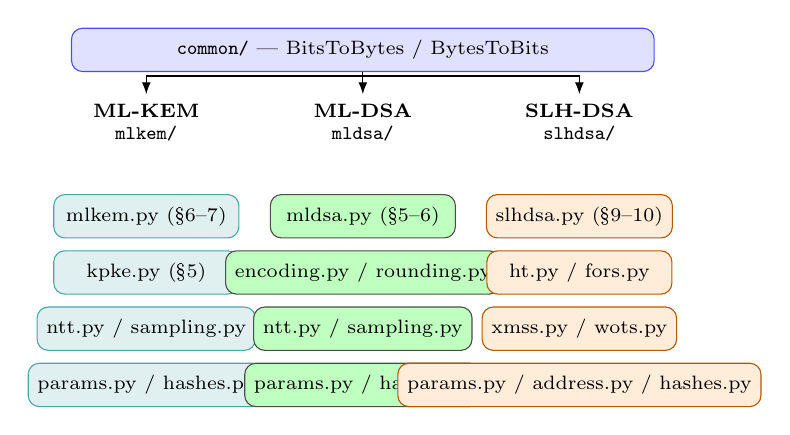
\begin{tikzpicture}[
  commonbox/.style={draw=blue!70, rounded corners, minimum width=7.4cm,
    minimum height=0.55cm, align=center, font=\scriptsize, fill=blue!12},
  kembox/.style={draw=teal!70, rounded corners, minimum width=2.35cm,
    minimum height=0.55cm, align=center, font=\scriptsize, fill=teal!12},
  dsabox/.style={draw=black!70, rounded corners, minimum width=2.35cm,
    minimum height=0.55cm, align=center, font=\scriptsize, fill=green!25},
  slhbox/.style={draw=orange!70!black, rounded corners, minimum width=2.35cm,
    minimum height=0.55cm, align=center, font=\scriptsize, fill=orange!15},
  lbl/.style={font=\scriptsize\bfseries, align=center}
]
\node[commonbox] (common) {\texttt{common/} --- BitsToBytes / BytesToBits};

\node[lbl, below=0.28cm of common, xshift=-2.75cm] (l1) {ML-KEM\\\texttt{mlkem/}};
\node[lbl, below=0.28cm of common, xshift=0cm]     (l2) {ML-DSA\\\texttt{mldsa/}};
\node[lbl, below=0.28cm of common, xshift=2.75cm]  (l3) {SLH-DSA\\\texttt{slhdsa/}};

\node[kembox, below=0.55cm of l1] (k4) {mlkem.py (\S6--7)};
\node[kembox, below=0.15cm of k4] (k3) {kpke.py (\S5)};
\node[kembox, below=0.15cm of k3] (k2) {ntt.py / sampling.py};
\node[kembox, below=0.15cm of k2] (k1) {params.py / hashes.py};

\node[dsabox, below=0.55cm of l2] (d4) {mldsa.py (\S5--6)};
\node[dsabox, below=0.15cm of d4] (d3) {encoding.py / rounding.py};
\node[dsabox, below=0.15cm of d3] (d2) {ntt.py / sampling.py};
\node[dsabox, below=0.15cm of d2] (d1) {params.py / hashes.py};

\node[slhbox, below=0.55cm of l3] (s4) {slhdsa.py (\S9--10)};
\node[slhbox, below=0.15cm of s4] (s3) {ht.py / fors.py};
\node[slhbox, below=0.15cm of s3] (s2) {xmss.py / wots.py};
\node[slhbox, below=0.15cm of s2] (s1) {params.py / address.py / hashes.py};

\draw[-{Latex[length=1.5mm]}] (common.south) -- ++(0,-0.05) -| (l1);
\draw[-{Latex[length=1.5mm]}] (common.south) -- (l2);
\draw[-{Latex[length=1.5mm]}] (common.south) -- ++(0,-0.05) -| (l3);
\end{tikzpicture}
\caption{Repository dependency structure: three parallel, bottom-up
module stacks (ML-KEM, ML-DSA, SLH-DSA), each depending only on layers
below it, sharing a single genuinely-duplicated primitive
(\texttt{common/}). ML-KEM and ML-DSA additionally share the NTT/lattice
style of construction (though with different moduli and root-of-unity
structure, so the code itself is not shared); SLH-DSA shares nothing
lattice-related, being purely hash-based.}
\label{fig:arch}
\end{figure}

Figure~\ref{fig:arch} summarizes the repository's parallel structure.
Each of the three algorithm packages is a self-contained, bottom-up
dependency stack: a \texttt{params.py} module holding the parameter
set's constants and derived sizes; primitive layers (byte/bit
conversion, hashing/XOF wrappers, NTT, sampling); and a top-level module
exposing the standard's public API (\texttt{KeyGen}/\texttt{Encaps}/
\texttt{Decaps} for ML-KEM; \texttt{KeyGen}/\texttt{Sign}/\texttt{Verify}
plus the pre-hash \texttt{HashML-DSA}/\texttt{HashSLH-DSA} variants for
the two signature schemes). This structure lets a reader trace any
top-level operation down to the exact FIPS algorithm and section
implementing each step, module by module.

\subsection{ML-KEM and ML-DSA: Shared Construction Style, Different Rings}

ML-KEM and ML-DSA both operate over polynomial rings of the form
$R_q = \mathbb{Z}_q[X]/(X^{256}+1)$ and both use a Number-Theoretic
Transform (NTT) to accelerate polynomial multiplication, but the two
rings differ in a way that changes the NTT's structure entirely.
ML-KEM's modulus $q = 3329$ has a primitive \emph{256th} root of unity
$\zeta = 17$, so $X^{256}+1$ factors into 128 \emph{quadratic} factors;
NTT-domain polynomial multiplication therefore requires a base-case
multiplication step (Algorithm 12 of FIPS 203) operating on
degree-1 pairs. ML-DSA's modulus $q = 8{,}380{,}417 = 2^{23} - 2^{13} + 1$
has a primitive \emph{512th} root of unity $\zeta = 1753$, so
$X^{256}+1$ factors completely into 256 \emph{linear} factors; the
ML-DSA NTT is fully diagonal, and multiplication in the NTT domain is a
simple element-wise (pointwise) product. This distinction --- verified
directly in our test suite via the identity $\zeta^{256} \equiv -1
\pmod q$ for ML-DSA --- is a recurring point of confusion when porting
lattice-scheme code between the two standards and is documented
explicitly in our project conventions as a common source of bugs.

\subsection{Hardware: A Shared Keccak/SHA-3/SHAKE Accelerator}

All three standards bottom out in the same cryptographic primitive:
Keccak-f[1600], the permutation underlying SHA-3 and SHAKE (FIPS 202
\cite{fips202}). ML-KEM uses SHA3-256/512 and SHAKE-128/256; ML-DSA uses
SHAKE-256 and SHAKE-128; SLH-DSA uses SHAKE-256 for \emph{every} one of
its six hash functions ($F$, $H$, $T_\ell$, $\mathrm{PRF}$,
$\mathrm{PRF\_msg}$, $\mathrm{H\_msg}$), regardless of the ``128'' in its
parameter-set name, which denotes classical security level rather than
XOF variant. One permutation core plus a parameterizable sponge (rate,
domain-separation byte, and fixed-output vs.\ XOF mode) therefore covers
every hash/XOF call made anywhere in the software reference
implementation, making it the highest-leverage first target for hardware
exploration.

We implemented, in SystemVerilog, a synthesizable, simulation-verified
Keccak-f[1600]/SHA-3/SHAKE core (\texttt{hardware/rtl/keccak/}):

\begin{itemize}
\item \texttt{keccak\_pkg.sv} --- lane/state typedefs, the 24
  round constants $RC[0..23]$, the $\rho$-offset table, and mode/rate/
  domain constants (FIPS 202 Table~1--2).
\item \texttt{keccak\_round.sv} --- one combinational round, the five
  step mappings $\theta, \rho, \pi, \chi, \iota$ (FIPS 202 \S3.2).
\item \texttt{keccak\_f1600.sv} --- the 24-round permutation, implemented
  as a one-round-per-cycle finite-state machine (the clearest mapping to
  FIPS 202 and easiest to verify; unrolling/pipelining is explicitly
  deferred pending a measured performance need).
\item \texttt{keccak\_sponge.sv} --- byte-serial absorb with
  domain-separated $\mathrm{pad10^{*}1}$ padding, permute, and squeeze,
  parameterized by rate and domain byte (FIPS 202 \S4, Algorithm~8).
\item \texttt{shake\_xof.sv} --- a mode-select wrapper selecting rate,
  domain byte, and fixed/XOF output mode for SHAKE128, SHAKE256,
  SHA3-256, and SHA3-512 (FIPS 202 \S6).
\end{itemize}

The Python reference implementation's own hash wrappers (already
cross-checked against the NIST KATs) serve as the golden model: a vector
generator (\texttt{hardware/tb/vectors/gen\_vectors.py}) exports
per-mode stimulus/expected-digest pairs from Python's \texttt{hashlib},
which a self-checking Icarus Verilog testbench
(\texttt{hardware/tb/smoke/}) replays against the RTL with no live
Python process required during simulation --- keeping the hardware
regression fast and dependency-free. A parallel UVM testbench skeleton
(\texttt{hardware/tb/keccak/}) is scaffolded for a full commercial-simulator
verification flow (Questa/VCS/Xcelium) in a later phase.

\subsection{Interactive Visualizations}

To make each standard's internal structure concrete and explorable, we
built four self-contained, dependency-free HTML/SVG/JavaScript
visualizations under \texttt{visualization/}: one per algorithm
(\texttt{slh-dsa.html}, \texttt{mldsa.html}, \texttt{mlkem.html}) plus an
overview/comparison hub (\texttt{index.html}). Each per-algorithm page
exposes several interactive tabs walking through that scheme's specific
structure --- for example, ML-DSA's page lets a reader click into any
cell of the $\hat A$ matrix to see its exact seed-derivation formula, or
step through the eight stages of the Sign rejection loop (Algorithm~7)
with a synchronized diagram highlighting the active components at each
step --- and a parameter-set selector so the same page can display every
NIST-defined variant of that standard. All four pages cross-link via a
consistent ``Algorithm'' dropdown in the navigation bar, and the overview
hub aggregates the cross-scheme size comparison presented in
Section~VI-C.

\section{Technical Details}

\subsection{FIPS 203: ML-KEM}

ML-KEM's security reduces to Module-LWE hardness. The scheme is built in
two layers: an underlying public-key encryption scheme, K-PKE (FIPS 203
\S5, Algorithms~13--15), and a KEM wrapper (FIPS 203 \S6--7,
Algorithms~16--21) built from K-PKE via a Fujisaki--Okamoto-style
transform that additionally provides \emph{implicit rejection}.

\textbf{K-PKE.} \texttt{KeyGen} samples a public matrix
$\hat A \in T_q^{k \times k}$ from a public seed $\rho$ via rejection
sampling (\texttt{SampleNTT}, Algorithm~7) and secret/error vectors
$s, e$ from a centered binomial distribution (\texttt{SamplePolyCBD},
Algorithm~8), then computes the public key $t = \hat A \circ \hat s + \hat
e$ (in the NTT domain) and secret key $s$. \texttt{Encrypt} samples a
fresh randomness vector, forms $u = \hat A^T \circ \hat r + e_1$ and
$v = t^T \circ \hat r + e_2 + \mathrm{Decompress}(m)$, and compresses
$(u, v)$ lossily to shrink the ciphertext (Compress/Decompress, FIPS 203
\S4.2.1). \texttt{Decrypt} recovers an approximation of the message from
$v - s^T u$ and decodes it.

\textbf{ML-KEM.} The KEM wrapper's \texttt{KeyGen} derives $(z, K\text{-PKE
keys})$ from a seed and stores $z$ (used only for implicit rejection);
\texttt{Encaps} derives message randomness deterministically from a hash
of the encapsulation key and a fresh random value, so that the same
$(ek, m)$ pair always produces the same ciphertext and shared secret,
closing a category of chosen-ciphertext attacks; \texttt{Decaps}
re-encrypts the recovered plaintext and compares ciphertexts in constant
time --- on mismatch, it does not raise an exception but instead returns
$J(z \| c)$, a pseudorandom value indistinguishable from a genuine shared
secret to an attacker without $z$. \S7 additionally mandates explicit
input-validation checks: an encapsulation-key type/modulus check (via a
decode/re-encode round-trip) and a decapsulation-key type/hash check
(recomputing $H(ek)$ and comparing against the value embedded in $dk$).

\subsection{FIPS 204: ML-DSA}

ML-DSA's security reduces to Module-SIS hardness and follows the
Fiat--Shamir-with-aborts paradigm for turning an interactive
identification scheme into a non-interactive signature.

\textbf{KeyGen (Algorithm~6).} Two small secret vectors $s_1 \in R_q^\ell$,
$s_2 \in R_q^k$ are sampled from a seed via rejection sampling
(\texttt{ExpandS}), and the public key is computed as
$t = \hat A \cdot \hat s_1 + s_2$, where $\hat A \in T_q^{k \times \ell}$
is expanded from a public seed $\rho$ (\texttt{ExpandA}). $t$ is then
split via \texttt{Power2Round} into a coarse public component $t_1$
(published as part of the public key) and a fine secret component $t_0$
(retained in the secret key), reducing public-key size at the cost of
retaining extra secret state needed during signing.

\textbf{Sign (Algorithm~7).} The signer commits to a random masking
vector $y$ with coefficients in $(-\gamma_1, \gamma_1]$
(\texttt{ExpandMask}), computes $w = \hat A \cdot \hat y$, and extracts
its high-order bits $w_1$ via \texttt{HighBits} (discarding the
low-order bits, which are never transmitted directly). The message is
hashed together with $w_1$ to derive a challenge seed
$\tilde c = H(\mu \| w_1\mathrm{Encode}(w_1))$, which is expanded into a
sparse polynomial $c$ with exactly $\tau$ nonzero $\pm 1$ coefficients
(\texttt{SampleInBall}, Algorithm~29) --- a Fisher--Yates-style sampler
over the polynomial's 256 coefficients. The response is
$z = y + c \cdot s_1$. Crucially, the signer then checks four bounds ---
$\|z\|_\infty < \gamma_1 - \beta$,
$\|\mathrm{LowBits}(w - c s_2)\|_\infty < \gamma_2 - \beta$,
$\|c \cdot t_0\|_\infty < \gamma_2$, and a maximum total hint weight
$\leq \omega$ --- and \emph{restarts signing from scratch with a fresh
$y$} if any bound is violated. This rejection-sampling loop is what makes
the signature's distribution independent of the secret key: an
accepted $z$ leaks (in the information-theoretic sense used in the
security proof) essentially nothing about $s_1$, because every value in
the accepted range was reachable regardless of the secret. The final
signature bundles $\tilde c$, $z$, and a compact 1-bit-per-coefficient
\emph{hint} $h$ that lets the verifier reconstruct $w_1$ without the
signer ever transmitting $w$'s low-order bits directly.

\textbf{Rounding and hints (Algorithms~35--40).} The
\texttt{Decompose}/\texttt{HighBits}/\texttt{LowBits} family splits a
ring element $r \equiv r_1 \cdot (2\gamma_2) + r_0 \pmod q$ with
$r_0 \in (-\gamma_2, \gamma_2]$, including a wraparound special case at
$r = q-1$ that forces $r_1 = 0$. \texttt{MakeHint}/\texttt{UseHint}
implement the load-bearing identity
$\mathrm{UseHint}(\mathrm{MakeHint}(z, r), r) = \mathrm{HighBits}(r+z)$
for $|z| \leq \gamma_2$: the signer sends a single bit indicating whether
adding $z$ crossed a bucket boundary, and the verifier --- who has $r$
but not $z$ --- can exactly recover $\mathrm{HighBits}(r+z)$ from that
one bit alone. This mechanism is what allows ML-DSA to omit $w$'s
low-order bits from the signature entirely while still letting the
verifier recompute the exact commitment needed to re-derive and check
$\tilde c$.

\textbf{Verify (Algorithm~8).} The verifier recomputes
$\hat A \cdot \hat z - \hat c \cdot \hat t_1 \cdot 2^d$, applies
\texttt{UseHint} with the transmitted hints to recover $w_1'$, re-derives
the challenge hash from $w_1'$, and accepts only if it matches $\tilde c$
and $\|z\|_\infty < \gamma_1 - \beta$. Forging a signature without the
secret key would require finding a short $z$ satisfying the public
Module-SIS relation directly --- exactly the hard problem the scheme's
security reduces to.

\subsection{FIPS 205: SLH-DSA}

SLH-DSA composes the four hash-based primitives introduced in
Section~II-C. \texttt{WOTS+} signs a single message digit-by-digit by
revealing intermediate points along $\mathrm{LEN}$ hash chains, each of
length $w$ (16 for our chosen parameter set); the signature for digit
$d_i$ is the chain value at step $d_i$, and verification applies the
chain function $F$ the remaining $w-1-d_i$ times, checking the result
against the stored public-key chain top. \texttt{XMSS} authenticates
$2^{h'}$ WOTS+ key pairs under a single Merkle root by including, with
each signature, the $h'$ sibling nodes (the \emph{authentication path})
needed to recompute that root from the signed leaf. The
\texttt{hypertree} stacks $D$ layers of XMSS trees, where layer $0$
signs the FORS public key and each higher layer signs the XMSS root of
the layer below, extending authentication to $D \times h'$ total bits of
address space without requiring an impractically tall single tree.
\texttt{FORS} signs the (large) message digest itself by splitting it
into $K$ independent $A$-bit indices, one per FORS tree, and revealing
each tree's secret leaf plus its authentication path; the $K$ recovered
tree roots are compressed with a further hash into the single FORS
public key that the hypertree ultimately signs. Every hash call in this
composition is domain-separated by a 32-byte \texttt{ADRS} structure
whose type-specific fields change meaning by ADRS type (seven types are
defined), preventing any single hash output from being valid in more
than one structural role.

\subsection{Correctness Bugs Discovered and Fixed}

Two non-trivial correctness issues surfaced during development, both
instructive about the limits of self-consistency testing.

\textbf{ML-DSA centered $\ell_\infty$-norm bug.} An early implementation
of the centered infinity-norm helper used the naive formula
$\max(\min(c,\, q-c))$ to convert a coefficient into its
$[0, q/2]$-centered absolute value. This formula silently drops the
negative side of coefficients already given in \emph{signed} form (as
\texttt{LowBits} returns them, in $(-\gamma_2, \gamma_2]$), as opposed to
coefficients given in mod-$q$ form ($[0, q)$), which the sampler/NTT
pipeline otherwise produces. Because Sign's $\|r_0\|_\infty < \gamma_2 -
\beta$ rejection check only constrained the positive half of the
coefficient range under this bug, it occasionally accepted signatures
that in fact violated the
$\mathrm{HighBits}(w - c s_2) = \mathrm{HighBits}(w)$ invariant Verify
depends on, silently breaking verification on roughly 2.5\% of random
sign/verify round-trips. Every fixed NIST KAT vector happened to avoid
triggering the bug; it was caught only by our in-house property tests,
which exercise 500 randomized round-trips per run. The fix canonicalizes
either input representation into $(-q/2,\, q/2]$ before taking the
absolute value, after which 0/500 randomized round-trips fail.

\textbf{SLH-DSA wrong XOF variant.} FIPS 205 \S10.2 fixes SHAKE256 for
\emph{every} SHAKE-based parameter set's six hash functions, regardless
of the ``128''/``192''/``256'' security-level designator in the
parameter-set name --- that number denotes classical security strength,
not the XOF variant. An early implementation instantiated
$F, H, T_\ell, \mathrm{PRF}, \mathrm{PRF\_msg}, \mathrm{H\_msg}$ with
SHAKE128 instead. Because Sign and Verify used the same (wrong) hash
function consistently with each other, every internal round-trip test
passed --- self-consistent code that agrees with itself is not evidence
of correctness against an external specification. The bug was invisible
until it was checked against an independent oracle: the first NIST ACVP
KAT run failed every single KeyGen vector. After correcting the hash
instantiation to SHAKE256, all 181 SLH-DSA tests (76 KATs plus 105
in-house) passed.

Both incidents reinforce the same lesson, and motivated our two-tier
verification strategy: self-consistent internal testing (unit tests,
round-trip property tests) is necessary but not sufficient, because a
bug that both the signer and verifier share consistently is invisible to
any test that only checks agreement between the two. Only an independent
external reference --- here, NIST's ACVP KAT vectors --- reliably
surfaces this class of error.

\section{Results, Evaluation, and Discussion}

\subsection{Test Suite Results}

\begin{table}[!t]
\caption{Test Suite Results by Scheme}
\label{tab:tests}
\centering
\begin{tabular}{lrrr}
\toprule
Scheme & NIST ACVP KATs & In-house & Total \\
\midrule
ML-KEM-768 (FIPS 203)         & 80  & 73  & 153 \\
ML-DSA-65 (FIPS 204)          & 115 & 119 & 234 \\
SLH-DSA-SHAKE-128s (FIPS 205) & 76  & 105 & 181 \\
\midrule
\textbf{Total}                & \textbf{271} & \textbf{297} & \textbf{568} \\
\bottomrule
\end{tabular}
\end{table}

Table~\ref{tab:tests} summarizes our full test suite. All 568 tests
pass, of which 271 are byte-for-byte NIST ACVP vectors spanning key
generation, encapsulation/signing, decapsulation/verification, and (for
ML-KEM) the \S7 encapsulation-/decapsulation-key validity checks. The
ML-KEM-768 vectors cover 25 KeyGen, 25 encapsulation, 10 decapsulation,
10 encapsulation-key-check, and 10 decapsulation-key-check cases. The
ML-DSA-65 vectors cover 25 KeyGen plus 60 signature-generation and 30
signature-verification cases spanning both pure ML-DSA and the
pre-hashed HashML-DSA variant, in both deterministic and hedged
(randomized) signing modes. The SLH-DSA-SHAKE-128s vectors cover 10
KeyGen, 38 signature-generation, and 28 signature-verification cases,
similarly spanning deterministic and hedged modes, restricted to the
implemented SHAKE/``s''/external-interface configuration. Passing every
KAT vector is, per our verification methodology (Section~III-D), the
authoritative evidence that our implementation faithfully realizes each
FIPS standard; the in-house tests provide a complementary regression net
and, as Section~V-D shows, were essential to catching at least one bug
the KATs alone did not expose during initial development.

\subsection{Hardware Accelerator Status}

The Keccak-f[1600]/SHA-3/SHAKE core has completed its first two of four
planned phases. \texttt{keccak\_round} and \texttt{keccak\_f1600} are
implemented and verified against a known reference state (an all-zero
input permutes to lane $[0][0] = \mathtt{0xF1258F7940E1DDE7}$, with the
\texttt{done} signal asserting after 25 cycles, consistent with a
one-round-per-cycle, 24-round permutation plus one setup cycle).
\texttt{keccak\_sponge} and \texttt{shake\_xof} are implemented and pass
a self-checking Icarus Verilog smoke test across all four target modes
(SHA3-256, SHA3-512, SHAKE128, SHAKE256), including multi-block absorb
(200-byte input) and multi-block squeeze (168- and 300-byte XOF output),
verified against Python \texttt{hashlib} golden vectors. The full UVM
verification environment (directed and randomized sequences, a KAT-file-driven
scoreboard, and mode$\times$length coverage) remains scaffolded but not
yet fleshed out, and downstream datapaths (an NTT unit for ML-KEM/ML-DSA;
WOTS+/XMSS/FORS hash chains for SLH-DSA) have not yet begun --- both are
discussed as future work in Section~VIII.

\subsection{Cross-Scheme Size Comparison}

\begin{table}[!t]
\caption{Sizes of the Three Parameter Sets Implemented in This Repository}
\label{tab:headline}
\centering
\begin{tabular}{lrrr}
\toprule
Scheme (parameter set) & Public key & Secret key & Primary artifact \\
\midrule
ML-KEM-768  & 1{,}184 B & 2{,}400 B & 1{,}088 B (ciphertext) \\
ML-DSA-65   & 1{,}952 B & 4{,}032 B & 3{,}309 B (signature) \\
SLH-DSA-128s&    32 B &    64 B & 7{,}856 B (signature) \\
\bottomrule
\end{tabular}
\end{table}

\begin{table}[!t]
\caption{Primary Artifact Size Across All Size-Distinct Parameter Sets,
Sorted Descending. SHA2 and SHAKE Variants of the Same Security
Level/Speed Are Byte-Identical and Shown Once. Implemented Sets in Bold.}
\label{tab:allvariants}
\centering
\begin{tabular}{lrrr}
\toprule
Parameter set & Public key & Secret key & Primary artifact \\
\midrule
SLH-DSA-256f     & 64 B    & 128 B   & 49{,}856 B \\
SLH-DSA-192f     & 48 B    & 96 B    & 35{,}664 B \\
SLH-DSA-256s     & 64 B    & 128 B   & 29{,}792 B \\
SLH-DSA-128f     & 32 B    & 64 B    & 17{,}088 B \\
SLH-DSA-192s     & 48 B    & 96 B    & 16{,}224 B \\
\textbf{SLH-DSA-128s} & \textbf{32 B} & \textbf{64 B} & \textbf{7{,}856 B} \\
ML-DSA-87        & 2{,}592 B & 4{,}896 B & 4{,}627 B \\
\textbf{ML-DSA-65} & \textbf{1{,}952 B} & \textbf{4{,}032 B} & \textbf{3{,}309 B} \\
ML-DSA-44        & 1{,}312 B & 2{,}560 B & 2{,}420 B \\
ML-KEM-1024      & 1{,}568 B & 3{,}168 B & 1{,}568 B \\
\textbf{ML-KEM-768} & \textbf{1{,}184 B} & \textbf{2{,}400 B} & \textbf{1{,}088 B} \\
ML-KEM-512       & 800 B   & 1{,}632 B & 768 B \\
\bottomrule
\end{tabular}
\end{table}

Tables~\ref{tab:headline} and \ref{tab:allvariants} present a
cross-scheme comparison of public-key, secret-key, and primary-artifact
(ciphertext, for the KEM; signature, for the two signature schemes)
sizes, computed directly from each standard's parameter definitions and
cross-checked against the byte sizes our implementation produces. Note
that a KEM ciphertext and a digital signature are different kinds of
object; we present them together, in the same unit (bytes transmitted
per operation), for scale comparison rather than as a like-for-like
substitute.

The comparison makes the central size trade-off between lattice-based
and hash-based post-quantum signatures concrete: at a comparable NIST
security category, SLH-DSA-128s's 7,856-byte signature is roughly 2.4
times the size of ML-DSA-65's 3,309-byte signature and roughly 7.2 times
the size of ML-KEM-768's 1,088-byte ciphertext, despite SLH-DSA-128s
having a \emph{dramatically smaller} key pair (32/64 bytes versus
1,952/4,032 bytes for ML-DSA-65) --- a direct consequence of SLH-DSA's
public key being only a short hash-tree root and PRF seed, with no
lattice matrix to encode. At the higher end, SLH-DSA-256f's 49,856-byte
signature is approximately 65 times the size of ML-KEM-512's 768-byte
ciphertext. This size profile is precisely why FIPS 205 is generally
positioned as a conservative, hash-based fallback rather than a default
choice for bandwidth-constrained deployments: its security rests on
weaker, more conservative assumptions (hash-function one-wayness rather
than a comparatively young lattice hardness assumption), at the direct
cost of signature size, while its extremely small key pairs make it
attractive wherever key size, rather than signature size, is the binding
constraint.

\subsection{Discussion: Were the Project's Objectives Achieved?}

Against the objectives set out at project start, we achieved full
implementation and NIST ACVP validation of one parameter set per
standard (Table~\ref{tab:tests}), which was the project's primary,
highest-priority goal. We additionally completed meaningful early
progress on two originally-stretch objectives: a functional (if partial)
hardware accelerator for the primitive shared by all three schemes, and
a set of interactive teaching visualizations that were not part of the
original project plan at all but emerged naturally from the team's own
need to build intuition for each standard's internal structure --- and
which directly enabled the quantitative size comparison in
Section~VI-C. The originally planned cross-algorithm runtime/complexity
performance analysis, and support for additional parameter sets beyond
the one chosen per standard, remain incomplete and are discussed in
Section~VIII as the primary remaining work.

\subsection{Development Challenges and Team Reflection}

Two practical challenges shaped how this project unfolded. First,
implementing the three standards --- which we initially expected to be
the largest share of the project's effort --- turned out, with heavy use
of an LLM coding assistant (Claude Code), to be one of the faster parts
of the work; the harder and more time-consuming part was, and remains,
building genuine understanding of the underlying lattice mathematics,
hash-tree constructions, and quantum-computing threat model well enough
to explain \emph{why} each line of pseudocode is there, not merely that
it reproduces NIST's expected output. This is a meaningful shift from
how a project like this would have been scoped even a few years ago: the
bottleneck moved from ``can we get this to run correctly'' to ``do we
understand it well enough to reason about it,'' which is precisely the
gap our two-tier verification methodology (Section~III-D) and our
interactive visualizations (Section~IV-D) were built to help close for
the team itself, not only for an external reader. Second, coordinating a
team of graduate distance students across different work schedules and
time zones proved harder than any individual technical task; regular
asynchronous communication (Discord, GroupMe) and a standing weekly
meeting were what kept work distributed and moving, rather than any
single scheduling tool or process. Team composition also changed over
the course of the project, which required redistributing ownership of
in-progress work (notably the ML-DSA package) without losing momentum.
Both observations are consistent with what we reported at the project's
mid-point and held true through to this stage of the work.

\section{Conclusion}

We presented the design, implementation, and verification of a
from-scratch, spec-faithful Python reference implementation of all three
NIST-finalized Post-Quantum Cryptography standards --- ML-KEM-768,
ML-DSA-65, and SLH-DSA-SHAKE-128s --- prioritizing auditability over
performance so that each module can be checked against its corresponding
FIPS pseudocode section directly. Our implementation passes all 568
tests, including all 271 official NIST ACVP Known-Answer Test vectors
across the three schemes, and we documented two non-trivial correctness
bugs whose discovery illustrates why independent-reference validation
(not merely internal self-consistency) is necessary for cryptographic
software. We further built an early-stage SystemVerilog hardware
accelerator for the Keccak permutation shared by all three standards,
four interactive browser-based visualizations of each scheme's internal
structure, and a quantitative cross-scheme comparison showing that, at
comparable NIST security categories, hash-based SLH-DSA signatures are
roughly 2--65 times larger than lattice-based ML-DSA signatures or
ML-KEM ciphertexts, in exchange for a smaller key pair and a more
conservative hardness assumption. All source code, tests, hardware RTL,
and visualizations are publicly available in our GitHub repository
\cite{repo}.

\section{Future Work}

Several directions remain, roughly in priority order:

\begin{itemize}
\item \textbf{Runtime and complexity benchmarking.} The originally
  planned cross-algorithm and cross-parameter-set performance comparison
  (wall-clock time and asymptotic operation counts for KeyGen/
  Encaps-Sign/Decaps-Verify) has not yet been carried out and remains
  the most significant piece of unfinished scope.
\item \textbf{Additional parameter sets.} Most modules are already
  parameter-driven; extending coverage to ML-KEM-512/1024, ML-DSA-44/87,
  and the remaining eleven SLH-DSA variants (both ``f'' speed variants
  and the SHA2 hash instantiation) is expected to be comparatively
  mechanical, with the exception of SLH-DSA's SHA2 path, which requires
  new hash wiring rather than a parameter change alone.
\item \textbf{ML-DSA externalMu and SLH-DSA internal signing
  interfaces.} Both standards define an alternate signing entry point
  where the caller pre-computes and supplies the message digest rather
  than the raw message; we deliberately deferred both, as neither was
  needed for our current use case.
\item \textbf{Hardware acceleration, continued.} Complete the UVM
  verification environment (Phase 3) for the existing Keccak core; add
  an NTT datapath reusable by both ML-KEM and ML-DSA; add WOTS+/XMSS/FORS
  hash-chain datapaths for SLH-DSA, reusing the existing Keccak core;
  and eventually target an FPGA or ASIC backend beyond the current
  simulation-only scope.
\item \textbf{Hosting the visualization suite.} Enable GitHub Pages (or
  an equivalent static host) so the four interactive visualizations,
  currently runnable locally or via the repository's static files, are
  reachable at a stable public URL with working cross-page navigation.
\item \textbf{A CLI or higher-level KEM--DEM wrapper}, composing
  ML-KEM with a symmetric authenticated-encryption scheme to demonstrate
  an end-to-end hybrid encryption workflow rather than exposing only the
  raw KEM primitive.
\end{itemize}

\section*{Acknowledgment}

GenAI (Claude Code, Anthropic) was used extensively throughout this
project to accelerate implementation, assist with verification against
the FIPS pseudocode, and help draft sections of this report, consistent
with the disclosure in our earlier project documents. Every design
decision, generated section, and test result presented here was
reviewed and is understood by the team.

\begin{thebibliography}{00}

\bibitem{fips203} National Institute of Standards and Technology,
``Module-Lattice-Based Key-Encapsulation Mechanism Standard,'' FIPS PUB
203, Aug. 2024. [Online]. Available: \url{https://csrc.nist.gov/pubs/fips/203/final}

\bibitem{fips204} National Institute of Standards and Technology,
``Module-Lattice-Based Digital Signature Standard,'' FIPS PUB 204, Aug.
2024. [Online]. Available: \url{https://csrc.nist.gov/pubs/fips/204/final}

\bibitem{fips205} National Institute of Standards and Technology,
``Stateless Hash-Based Digital Signature Standard,'' FIPS PUB 205, Aug.
2024. [Online]. Available: \url{https://csrc.nist.gov/pubs/fips/205/final}

\bibitem{fips202} National Institute of Standards and Technology,
``SHA-3 Standard: Permutation-Based Hash and Extendable-Output
Functions,'' FIPS PUB 202, Aug. 2015. [Online]. Available:
\url{https://csrc.nist.gov/pubs/fips/202/final}

\bibitem{shor1997} P. W. Shor, ``Polynomial-Time Algorithms for Prime
Factorization and Discrete Logarithms on a Quantum Computer,'' \emph{SIAM
Journal on Computing}, vol. 26, no. 5, pp. 1484--1509, 1997.

\bibitem{nist-pqc} National Institute of Standards and Technology,
``Post-Quantum Cryptography Project.'' [Online]. Available:
\url{https://www.nist.gov/pqc}

\bibitem{nist-announce} National Institute of Standards and Technology,
``NIST Releases First 3 Finalized Post-Quantum Encryption Standards,''
Aug. 2024. [Online]. Available:
\url{https://www.nist.gov/news-events/news/2024/08/nist-releases-first-3-finalized-post-quantum-encryption-standards}

\bibitem{acvp} National Institute of Standards and Technology,
``ACVP-Server: Automated Cryptographic Validation Protocol Server and
Test Vectors.'' [Online]. Available:
\url{https://github.com/usnistgov/ACVP-Server}

\bibitem{peikert} C. Peikert, ``A Decade of Lattice Cryptography,''
\emph{Foundations and Trends in Theoretical Computer Science}, vol. 10,
no. 4, pp. 283--424, 2016.

\bibitem{pqclean} PQClean Project, ``PQClean: Clean, portable, tested
implementations of post-quantum cryptography.'' [Online]. Available:
\url{https://github.com/PQClean/PQClean}

\bibitem{liboqs} Open Quantum Safe Project, ``liboqs: C library for
quantum-resistant cryptographic algorithms.'' [Online]. Available:
\url{https://github.com/open-quantum-safe/liboqs}

\bibitem{repo} C. Kane, V. Kottapalli, and P. Marshall, ``CSCE 703 PQC
Standard Implementations,'' GitHub repository.
[Online]. Available:
\url{https://github.com/venky-k-tamu/csce703_project_summer_2026}

\end{thebibliography}

\end{document}
